\nocite{*} % cargar toda la bib
  \begin{abstract}
    La extinción de especies de animales en la actualidad genera impactos variados para el medio ambiente, desde la aparición de plagas hasta el desequilibrio ambiental. Uno de los grandes problemas que existen en la actualidad es la desaparición de depredadores tope el cual debido a su ausencia, el ecosistema donde residía tuvo un aumento de población de otras especies llegando a valores extremos y provocando el cambio del mismo. Ante esto se buscó resolver esta problemática a través de una técnica llamada “Rewilding” que consiste en la inserción de individuos provenientes de otras zonas en el ambiente donde estaba extinto para que este vuelva a poblar su lugar. Esto podría traer beneficios desde ambientales hasta la posibilidad de creación de parques turísticos donde la población de personas podría aprovechar esta oportunidad y crear una economía basada en el atractivo de la especie.
    En el presente estudio se buscará aplicar esta técnica con la especie animal conocida como Yaguareté o Jaguar el cual se encontraba extinto en los Esteros del Iberá (correspondiente a la provincia de Corrientes), cuyo trabajo de reinserción se está realizando actualmente. La idea principal del modelo de simulación es analizar el crecimiento de la población de esta especie según distintas variables, recreando zonas con distintas características que analizaremos en las siguientes secciones.
    De cada zona en estudio se analizará el comportamiento de cada individuo al cazar, reproducirse, territorialidad de individuos y crecimiento de las crías.

  \end{abstract}

    \keywords{rewilding \and yaguareté \and jaguar \and ambiente \and simulación \and iberá \and felinos \and animales \and ecosistema \and biología \and puma \and medioambiente}

\section{Introducción}
    Actualmente la población del yaguareté en la Argentina cuenta con aproximadamente 250 ejemplares, los cuales están distribuidos en distintas zonas del país. Por lo que la introducción de nuevos jaguares deberá tener en cuenta diversos factores para su introducción. En el caso de estudio se supondrá que se tienen 2 zonas posibles de inserción con distintas características y se deberán repartir entre 5 y 12 individuos en estas zonas de manera que puedan hacer crecer su población en un intervalo de tiempo de 10 años, sorteando los problemas que puedan surgir. Se tiene en cuenta la territorialidad propia de la especie no se pueden poner todos los ejemplares juntos en un una sola zona o en un lugar donde se cree que puede haber otros yaguaretés salvajes debido a que puede causar peleas entre su misma especie la cual ya se encuentra muy diezmada por causa del hombre.
    
    Otro punto a tener en cuenta es que se supondrá que los individuos a insertar han pasado yá un ciclo en el cual se da por hecho que pueden vivir en un ambiente salvaje y no han provenido previamente de un lugar donde convivieron con humanos (es decir, no fueron domesticados).

\section{Factores a analizar}
    Los factores a tener en cuenta para la simulación son los siguientes:
    
   \subsection{Capacidad de caza de un individuo}
    El yaguareté es un depredador hábil y eficiente. Su particularidad de ocupar amplios territorios le permite cazar pocas presas al mes, lo que logra evitar que el mismo acabe con su alimento. Además se encuentra al tope de la cadena alimenticia en sus hábitats por lo que no tiene competidores directos, exceptuando raras ocasiones en las que pueden surgir otros predadores como el puma, sin embargo, al ser casos aislados, no serán tenidos en cuenta en el estudio.
    
    Sus principales presas son el pecarí y la corzuela, aunque también se alimenta de carpinchos, tapires, agutíes, peces, reptiles, etc.
    
    \subsection{Reproducción y crianza}
    Debido a que su distribución abarca zonas muy amplias, parece no tener una época fija para criar.
    
    Luego de que un macho y una hembra se reproduzcan, la pareja se separa después de la cópula y, tras una gestación de 90 a 110 días la hembra busca una guarida donde dará a luz dos o tres cachorros, que pesan entre 600 y 900 gramos y mantienen los ojos cerrados hasta las dos semanas de vida. Su coloración es similar a la del adulto, pero parece más oscura pues las manchas son más confusas y más juntas entre sí. Puede pasar que en una misma camada nazcan cachorros manchados (pintados) y melánicos (negros).
    
    La madre es quien se ocupa de la crianza y se vuelve más agresiva para defender a sus cachorros. Durante los primeros días no se aleja mucho de sus hijos y, si no cree que estén seguros, las transporta con su boca hasta otro escondrijo. Durante este período la hembra restringe su área de movimiento y su territorio se achica temporalmente.
    
    Aproximadamente a los dos meses y medio empiezan a comer carne, a los tres dejan de mamar alimentándose exclusivamente de carne mientras que a los seis meses (a veces antes) abandonan su escondrijo para acompañar a su madre en sus salidas de caza. Finalmente, a los dos años de edad la madre los abandona para que comiencen una vida independiente: deberán encontrar y ganarse su propio territorio.
    
    El yaguareté alcanza su tamaño definitivo y su madurez sexual aproximadamente a la edad de tres años. En estado silvestre, viven hasta doce años, aunque hay algunos casos registrados recientemente de individuos más longevos (Link texto Nico Macho yanqui). En cautiverio en cambio, pueden superar los 20 años de edad. A lo largo de toda su vida una hembra puede dar a luz entre diez y doce cachorros.

    \subsection{Territorialidad}
    Sus territorios son amplios, pudiendo alcanzar hasta 30.000 hectáreas para machos adultos en zonas de condiciones de vida difíciles (alta intromisión humana, cacería, baja densidad de presas, etc), mientras que las hembras ocupan superficies menores (7-10 mil hectáreas) y se observa una gran diferencia entre diferentes tipos de ambientes.
    
    El Yaguareté es solitario. Cada macho establece su territorio expulsando a los otros, pero lo comparte con varias hembras, con las que se aparea. Las interacciones que ocurren por la conflictividad de los individuos y cómo afecta esto al crecimiento de la población y a la disponibilidad de terreno son factores fundamentales a tener en cuenta.
    
    \subsection{Mortalidad}
    Hay que tener en cuenta las causas más probables de la muerte de los yaguaretés, ya que es imperativo saber la esperanza de vida de estos animales si queremos una simulación útil. No solo hay que saber las causas sino también los efectos de tal suceso, para saber cómo modelar junto a sus implicaciones.
    
    Si bien una gran causa del fallecimiento de los individuos es por la amenaza humana ya sea por cazarlos o porque los territorios de la especie se ven disminuidos con fines comerciales o inmobiliarios. Al reducir el hábitat y ser una especie territorial, esto hace expulsar a los machos a zonas pobladas, lo que eleva el riesgo de ser asesinados.
    Además la infancia de los cachorros es complicada ya que se encuentran vulnerables, y si la madre no puede conseguirles suficiente comida o cuidarlos bien entonces estos pueden fallecer.

\section{Datos recolectados}
    \subsection{Capacidad de caza de un individuo}
    Se calcula que un yaguareté necesita cazar aproximadamente por semana un mínimo de 10,5 kg de presas. Por día se calcula que caza un promedio de 1.5 kg o 1.2 kg de presas o un poco más. Para este caso, se evalúa semanalmente si el individuo cazó menos de 10.5 kg de presas. Si es así el individuo fallece o en caso contrario se le quita un pesaje que usó para sobrevivir(se le quita un total de 8.5 kg de presas cazadas utilizadas para moverse, cazar otro animal o nadar).
    
    La distribución utilizada para ver la cantidad de presas que pudo haber cazado un yaguareté una distribución Normal con un desvío $\sigma$ =0.3 y una media $\mu$=1.5. Lo que nos deja una variable aleatoria continua distribuida normalmente denotada como:

    \begin{equation}
        X \sim N(\sigma=0.3, \mu=1.5)
    \end{equation}
    
    \subsection{Reproducción y crianza}
    
        \subsubsection{Frecuencia}
            Debido a que su distribución abarca zonas muy amplias, parece no tener una época fija para criar, aunque algunos estudios parecen indicar una tendencia más hacia la primavera en las zonas de condiciones climáticas más extremas, mientras que en áreas tropicales se reproduce en cualquier época del año. Otro dato que usaremos es que el yaguareté (tanto macho como hembra) alcanza su tamaño definitivo y su madurez sexual aproximadamente a la edad de dos años.
            
            Por lo que se calcula que una hembra tiene su época de celo cada cierto tiempo, en este caso nosotros utilizaremos un tiempo fijo aproximado de 75 días.
            
            El macho que se encuentre a unos 100 m de radio va a enterarse de la cercanía de una hembra y va a ir en su encuentro. Una vez cerca, la misma va embarazarse y luego de 100 días de gestación dará a luz una camada de hasta un máximo de 4 crías
        
        \subsubsection{Camadas}
            A lo largo de toda su vida una hembra puede dar a luz entre diez y doce cachorros, sin embargo las camadas son de entre 1 y 4 crías.
            
            La distribución de probabilidad utilizada aquí está inspirada en la encontrada en el paper “Análisis de la viabilidad de las poblaciones de jaguar: evaluación de parámetros y estudios de caso en tres poblaciones remanentes del sur de Sudamerica” (por Eduardo Eizirik, Cibele B. Indrusiak y Warren E . Johnson), la cual nos provee con las probabilidades de nacimiento de una determinada cantidad de cachorros por gestación:

            \begin{itemize}
                \item \textbf{1 cría:} 5\%
                \item \textbf{2 crías:} 40\%
                \item \textbf{3 crías:} 30\%
                \item \textbf{4 crías:} 25\%
            \end{itemize}
        \subsubsection{Sexo}
            Cada cachorro al momento de su nacimiento tiene una probabilidad de 0.5 de ser macho o hembra. Por lo que esta variable sigue un comportamiento binomial denotado de la siguiente manera:
            \begin{equation}
                X \sim B(n=1, p=0.5)
            \end{equation}
        \subsubsection{Sobrevivencia de cada cría en una camada}
            La sobrevivencia de cada cachorro como mencionamos anteriormente depende casi exclusivamente de la madre sin embargo puede suceder que los cachorros han nacido con enfermedades u otros impedimentos que puedan crecer y desarrollarse de manera efectiva. Se debe tener en cuenta el hábitat y la posibilidad de vivir con cachorros en la zona (puede haber inundaciones, poca agua, lugares con campos, etc.), y eso impacta en una tasa de mortalidad infantil.
            
            Los estudios indican que tienen una probabilidad de sobrevivencia en la época de crianza antes de separarse de su madre (dos años) de 0.25. Para representar esto, en el modelo de simulación utilizamos una variable aleatoria discreta con valores 0 y 1 con distribución binomial en el que si surge un 1, el cachorro fallece. Esta distribución se representa de la siguiente manera:

            \begin{equation}
                X \sim B(n=1, p=0.25)
            \end{equation}
            
    \subsection{Mortalidad}
        En estado silvestre, viven hasta doce años, aunque hay algunos casos registrados recientemente de individuos más longevos. En el modelo, hay un procedimiento que regularmente elimina a un yaguareté si tiene más de 15 años y luego de los 12 años el individuo tiene una probabilidad de 0.65 de fallecer por lo que el comportamiento de esta variable también sigue una distribución de probabilidad binomial denotada como:
        
        \begin{equation}
            X \sim B(n=1, p=0.65)
        \end{equation}

    \subsection{Territorialidad}
        Esta especie marca su territorio de distintas maneras, ya sea a través de excrementos, orina, afilandosé las uñas, etc. Estas marcas van desapareciendo a medida que pasa el tiempo por lo que cuando un macho se va por un tiemp de su territorio, otro aparece para poder reclamarlo como suyo.
        
        En caso de que uno se encuentre muy cerca de otro, hay una muy poca probabilidad de que ambos peleen porque esta especie trata de evitar estos conflictos. Sin embargo en el caso de que haya un encuentro uno de ellos morirá debido a la violenta pelea.
        La probabilidad de que esto suceda es de 0.15 por lo que volvemos a utilizar una distribución binomial para representarlo.
        
\section{Escenarios Planteados}
    \subsection{Escenario 1: Introducción de misma cantidad de machos y hembras}
        Este escenario contará con una introducción de 6 machos y 6 hembras en una zona con condiciones normales de presas y amenazas. Aquí todas sus características tendrán los valores previamente desarrollados y mencionados.
        
    \subsection{Escenario 2: Mayor cantidad de machos}
        En este escenario la cantidad de machos es superior, el doble de la cantidad de las hembras. Habrán 8 machos y 4 hembras.
        
    \subsection{Escenario 3: Menor cantidad de disponibilidad de presas y menor cantidad de supervivencia}
        En este último escenario se plantea una zona probablemente poblada por humanos en las que contará con una mortalidad promedio de 8 años. Esto es debido a la amenaza de represalias por parte del humano ya sea por haber cazado ganado vacuno o por el valor de su piel. Además contará con una menor disponibilidad de presas, por lo que cazará menos cantidad de la que necesita.
    
    
\section{Creación del modelo de simulación}
    Creamos la simulación en AnyLogic, realizando un modelo combinado orientado a agentes y eventos discretos. Consiste en un agente que representa al yaguareté macho y uno para la hembra, donde cada determinados intervalos de tiempo suceden distintos eventos los cuales según el comportamiento de cada sexo los agentes responden de distinta manera.
    
    Ambos tienen comportamientos de alimentación y reproducción. Pero hay otros comportamientos que son exclusivos de cada uno, el macho cuenta con un comportamiento territorial y la hembra con el embarazo y la época de crianza de los cachorros.


    El modelo de simulación tiene configurado el tiempo de configuración en días, los cuales cada paso es un día. Cada día los yaguaretés se mueven en una dirección específica cazando y marcando territorios. También son capaces de nadar y moverse hacia otros lugares por aguas no tan profundas. Además de esto, la herramienta permite generar aleatoriamente nuevas zonas al apretar un botón en el caso de que se requiera cambiar de mapa en el cual se encuentran los individuos actualmente.

    En base al objetivo, cada 10 años se inicia una nueva corrida guardando los datos de la simulación para luego ser usados en herramientas de estadísticas para poder llegar a una conclusión final en cuanto a los escenarios planteados previamente. Se planea conseguir 30 muestras de cada escenario para comparar resultados y definir cuál será la opción más óptima.
    
    Además de esto se puede monitorear de manera continua distintos parámetros a través de gráficos que se encuentran en el modelo. 
    Los mismos se pueden ver a continuación:
    
    \begin{figure}[!htb]
        \centering
        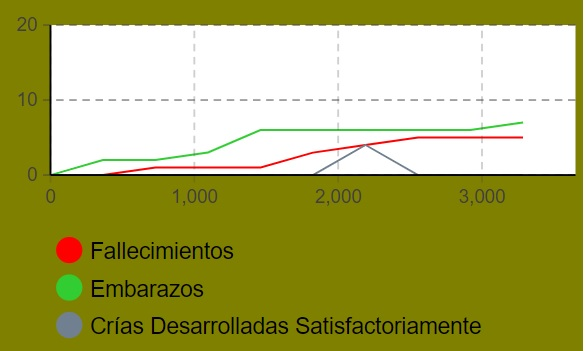
\includegraphics{imagen1.jpg}
        \caption{Cantidad de fallecimientos, embarazos y crías en total que se desarrollaron satisfactoriamente en la época de crianza}
        \label{fig:fig1}
        \bigskip
        \centering
        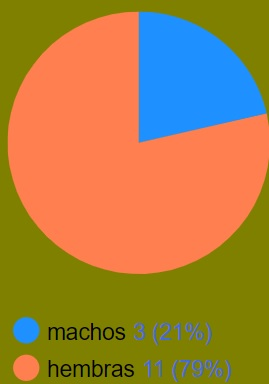
\includegraphics{imagen2.jpg}
        \caption{Cantidad de yaguaretés hembras en comparación con cantidad de machos}
        \label{fig:fig2}
        \bigskip
        \centering
        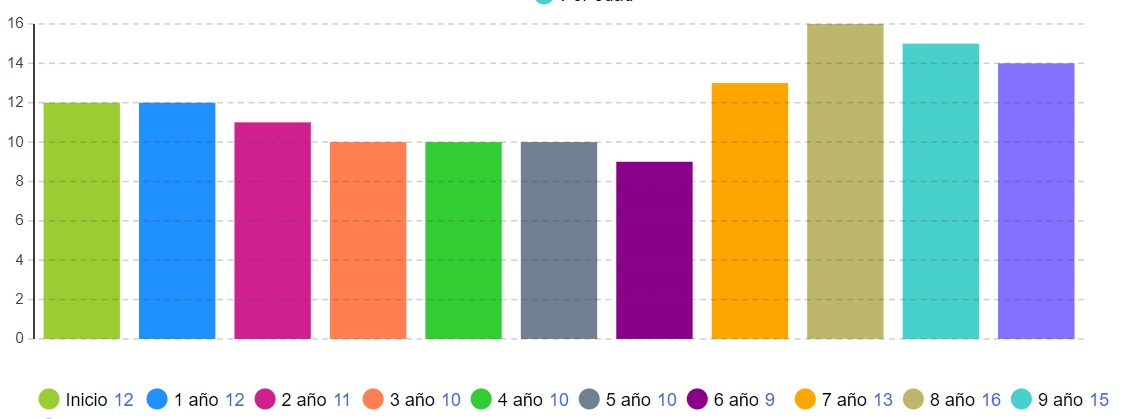
\includegraphics[width=350pt]{imagen4.jpg}
        \caption{Cantidad de individuos en el área por año}
        \label{fig:fig4}
    \end{figure}

\section{Resultados obtenidos}

    Recopilamos los datos en una planilla de MS Excel y representamos todas las corridas más la línea promedio.

    \subsection{Escenario 1}

    \begin{figure}[!htb]
        \minipage{0.32\textwidth}
        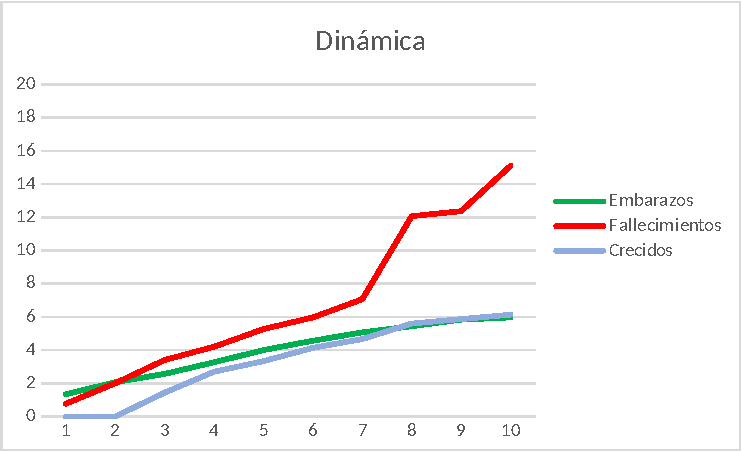
\includegraphics[width=\linewidth]{images/esc1/dinamica}
        \caption{Cantidad de fallecimientos, embarazos y crías en total que se desarrollaron satisfactoriamente en la época de crianza}\label{fig:fig1-1}
        \endminipage\hfill
        \minipage{0.32\textwidth}
        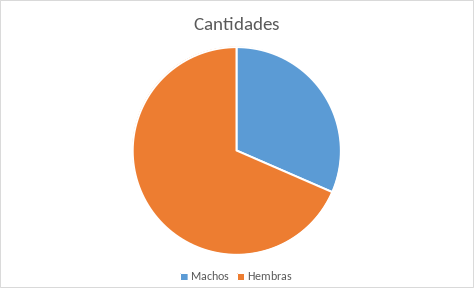
\includegraphics[width=\linewidth]{images/esc1/genero}
        \caption{Cantidad de yaguaretés hembras en comparación con cantidad de machos}\label{fig:fig1-2}
        \endminipage\hfill
        \minipage{0.32\textwidth}
        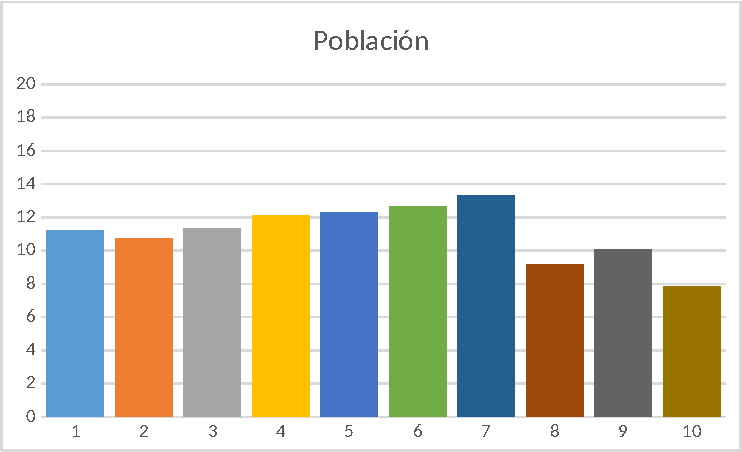
\includegraphics[width=\linewidth]{images/esc1/densidad}
        \caption{Cantidad de individuos en el área por año}\label{fig:fig1-3}
        \endminipage
    \end{figure}

    \subsection{Escenario 2}

    \begin{figure}[!htb]
        \minipage{0.32\textwidth}
        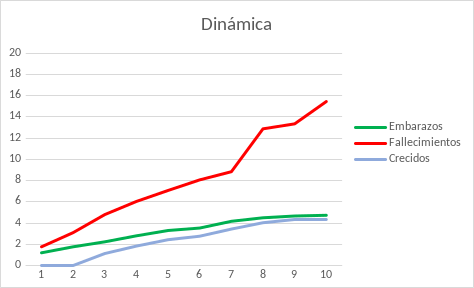
\includegraphics[width=\linewidth]{images/esc2/dinamica}
        \caption{Cantidad de fallecimientos, embarazos y crías en total que se desarrollaron satisfactoriamente en la época de crianza}\label{fig:fig2-1}
        \endminipage\hfill
        \minipage{0.32\textwidth}
        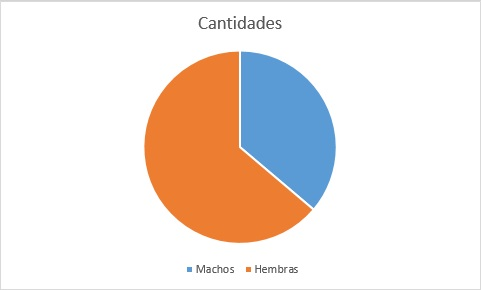
\includegraphics[width=\linewidth]{images/esc2/genero}
        \caption{Cantidad de yaguaretés hembras en comparación con cantidad de machos}\label{fig:fig2-2}
        \endminipage\hfill
        \minipage{0.32\textwidth}
        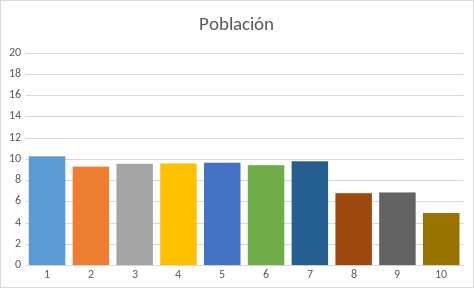
\includegraphics[width=\linewidth]{images/esc2/densidad}
        \caption{Cantidad de individuos en el área por año}\label{fig:fig2-3}
        \endminipage
    \end{figure}

    \subsection{Escenario 3}

    \begin{figure}[!htb]
        \minipage{0.32\textwidth}
        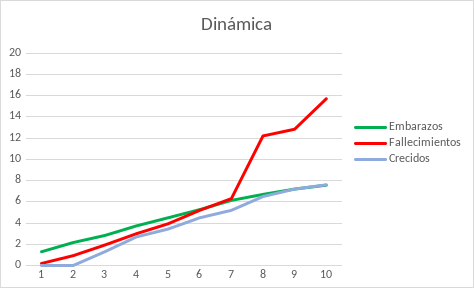
\includegraphics[width=\linewidth]{images/esc3/dinamica}
        \caption{Cantidad de fallecimientos, embarazos y crías en total que se desarrollaron satisfactoriamente en la época de crianza}\label{fig:fig3-1}
        \endminipage\hfill
        \minipage{0.32\textwidth}
        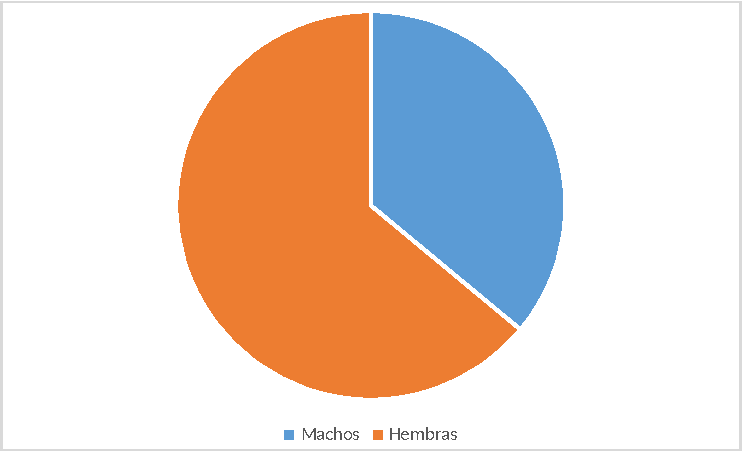
\includegraphics[width=\linewidth]{images/esc3/genero}
        \caption{Cantidad de yaguaretés hembras en comparación con cantidad de machos}\label{fig:fig3-2}
        \endminipage\hfill
        \minipage{0.32\textwidth}
        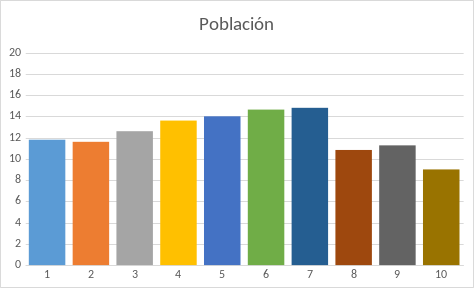
\includegraphics[width=\linewidth]{images/esc3/densidad}
        \caption{Cantidad de individuos en el área por año}\label{fig:fig3-3}
        \endminipage
    \end{figure}

    \section{Análisis estadísticos}
        En esta sección veremos los análisis a los resultados de los escenarios que hemos utilizado para llegar a un
        estimado de la población que puede llegar a tener en 10 años, estas zonas a las que hemos realizado
        el estudio. Esto también nos dará idea su cantidad de mortandad y/o embarazos, junto con la cantidad de crías que
        pueden llegar a crecer bajo determinadas condiciones iniciales.

        Para poder llegar a estos estimativos utilizaremos los siguientes dos análisis para así llegar a nuestro objetivo de
        verificar la supervivencia del yaguareté en estas zonas elegidas.

        \subsection{Intervalos de confianza t-apareado}

            La prueba de intervalos de confianza t-apareado nos dice que el escenario 2 es peor para la supervivencia de la especie.

            \begin{figure}[htbp]
                \centering
                \includegraphics{esc2/analisis.jpg}
                \caption{Conclusión del análisis por intervalos de confianza t-apareado comparando el escenario 2 con el 1.}
                \label{fig:fig1}
            \end{figure}

            El mismo análisis nos dice que en el escenario 3 la población al finalizar la simulación tiene una media
            similar al escenario 1, lo que significa que podemos esperar resultados similares en ambas condiciones.

            \begin{figure}[htbp]
                \centering
                \includegraphics{esc3/analisis.jpg}
                \caption{Conclusión del análisis por intervalos de confianza t-apareado comparando el escenario 3 con el 1.}
                \label{fig:fig1}
            \end{figure}

        \subsection{Intervalos de confianza 2t-muestras modificado}
            
\section{Conclusiones}

